% - Sicherheits-Applikation/ Spezielle Firewall
%    - Gefordert in diversen Compliance Richtlinien
% - was mach eine WAF im Prinzip?
%     - Zwischen Client und Server
%     - Analysiert Datenverkehr
% - Fokus auf web-Protokolle
%     - auf TCP/IP Layer 5
%     - HTTP, HTTPS, FTP
% - Traffic Analyse in Tiefe (Request & Response)
%     - HTTP (kapitel 5.2) beschreibt diverse Angriffswege
%     - Erkennung anhand von Regeln
%         - Black- vs. whitelisting
%         - Vordefiniertes Regelwerk
\label{chap:waf-theory}
Ein \ac{waf} ist eine Sicherheits-Applikation, die in der Lage ist den Datenverkehr zu und von einer Web-Anwendung zu Analysieren.
Hierbei werden die Übertragenen Inhalte in der Tiefe auf schädliche Inhalte überprüft.
Der in Abbildung \ref{fig:waf-porcess-flow} dargestellte Prozessablauf beschreibt wie eine \ac{waf} mit eingehenden Nachrichten umgeht.

\begin{figure}[!hbt]
    \centering
    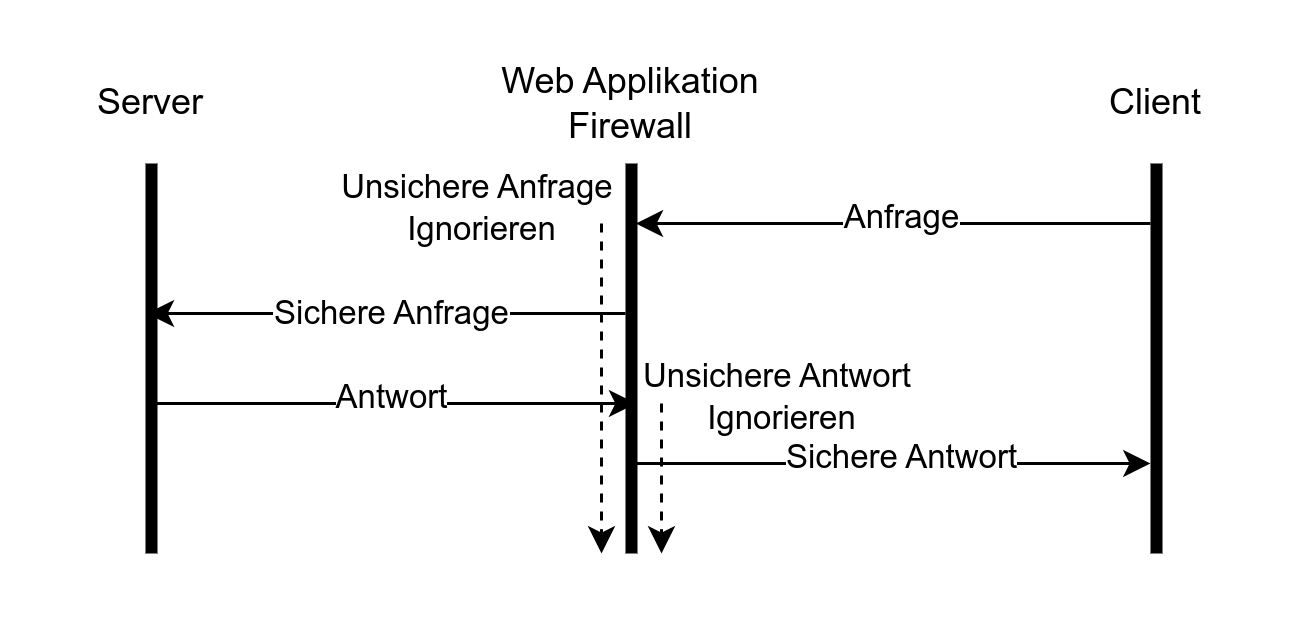
\includegraphics[width=0.9\textwidth]{./images/Waf-Process-fliow.png}
    \caption{Prozess Ablauf der Verarbeitung durch eine \ac{waf}}
    \label{fig:waf-porcess-flow}
\end{figure}

Das grundlegende Muster ist, dass einen Nachricht an der \ac{waf} eintrifft und von dieser an den Server weitergegeben wird.
Dieser Verarbeitete die Anfrage und sendet seine Antwort an die \ac{waf} die die Antwort an den Client weiterleitet.
Der Server kennt in diesem Muster den CLient nicht.
Die \ac{waf} ordnet der Anfrage die zugehörige Antwort zu.
Als schädlich erkannte Inhalte können sowohl in einer Anfrage als auch Antwort abgelehnt werden.
Anstatt einer abgelehnten Nachricht kann eine \ac{waf} auch eine eigene Antwort an den Client senden.
Das ermöglicht Nutzer festzustellen, dass ein Fehler in seiner Anfrage oder der Konfiguration der \ac{waf} vorliegt.
Mittels einer ID, die der ersetzten Antwort angehängt wird lässt sich das Verhalten im Nachhinein nachvollziehen
Neben den beiden Möglichkeiten weiterleiten und Ablehnen kann eine \ac{waf} die in einer Anfrage erkannten schädlichen Inhalte auch neutralisieren und die Nachricht weitergeben.

Eine \ac{waf} wird in produktiven Umgebungen in einem Netzwerk \textit{vor} den zu schützenden Anwendungen positioniert.
Das heißt der geschützte Server befindet sich in einer \ac{dmz}.
Eine \ac{dmz} ist ein, von anderen Netzwerkaktivitäten abgeschnittenes Netzwerksegment, das nur durch die \ac{waf} sowie weitere Sicherheitsanwendungen zugänglich ist.
Dadurch soll verhindert werden, dass ein Nutzer auf anderem Weg als vorgesehen Zugriff auf den Server erhält.

Neben den Klassischen Deployment-Methoden, bei denen die \ac{waf} als \ac{vm} oder Physischer Server im Unternehmensnetzwerk platziert ist, werden auch einige \ac{waf} als sogenannte \textit{Cloud-\ac{waf}} zur Verfügung gestellt.
Die \ac{waf} ist hier nicht im selben Netzwerk wie der Server sondern wird an anderer Stelle betrieben.
Dadurch ergeben sich einige Änderungen im Aufbau des Deployments:
Es muss sichergestellt werden, dass ein Client der eine Verbindung zum Server aufbauen möchte, bei der Namensauflösung (DNS) auf die \ac{waf} geleitet wird.
Der Server hingegen stellt sicher nur Verbindungen von der \ac{waf} zu akzeptieren.
Dies kann mit einer Firewall, die nur Verbindungen von der \ac{waf} akzeptiert, realisiert.
Es existieren auch Zertifikat basierte Verfahren, die die Authentizität der Datenherkunft sicherstellen.

Eine klassische Firewall nimmt Filterung auf Internet- und Transportschicht (Layer 2 und 3) des TCP/IP Modells vor.
Achtet also hauptsächlich auf IP-Adresse und Port Nummer.
Eine \ac{waf} hingegen arbeitet auf der Anwendungsschicht (Layer4).
Der Fokus liegt auf Internet-Protokollen wie HTTP und HTTPS. 
Aber auch Datentransferprotokolle wie FTP sind im Umfang einer \ac{waf}.

Da es sich bei HTTP und auch FTP um plaintext Protokolle handelt, bei denen der Datentransport in einer Menschenlesbarer Form erfolgt, unterscheidet sich die Funktion einer \ac{waf} grundsätzlich von der einer klassischen Firewall.
Die Erkennung schädlicher Inhalte erfolgen aufgrund von Regeln, die Muster beschreiben die auf schädliche Inhalte Hindeuten.
In der Implementierung wird dies in der Regel durch die Verwendung Regulärer Ausdrücke realisiert, diese bilden Muster ab die mit den Inhalten des Datenverkehrs abgeglichen werden.
Eine \ac{waf} muss jedes Datenpaket mit einer Anzahl von Regeln in der Größenordnung mehrerer hunderttausend bis Millionen regulärer Ausdrücke abgleichen.
Der Rechenaufwand kann zwar durch optimierte regex-Engines oder Tree-Pruning-Algorithmen die irrelevante Überprüfungspfade erkennen, verringert werden.
Jedoch ist der Rechenaufwand in einer \ac{waf} relativ hoch und die Hardware Anforderungen an eine \ac{waf} groß.
Auch muss bei einer vorgeschalteten \ac{waf} mit erhöhten antwortzeiten gerechnet werden, die sich im Millisekunden Bereich befindet.

Da es im Aktuellen stand der Technik üblich ist Internet-Datenübertragung zu verschlüsseln, muss eine \ac{waf} in der Lage sein die verschlüsselte Kommunikation zu öffnen um die Inhalte analysieren zu können.
Die SSL Verschlüsselung des HTTPS Protokolls wird also an der \ac{waf} terminiert.
Die Kommunikation zwischen Server \textit{hinter} der \ac{waf} und der \ac{waf} kann entweder unverschlüsselt oder mit einem separaten Satz Zertifikate erfolgen.
Die \ac{waf} verschlüsselt die Kommunikation nach der Verarbeitung wieder um sie an den Server weiterzugeben.
Die Abwägung ob in der \ac{dmz} verschlüsselt kommuniziert wird muss anhand von Compliance-Gesichtspunkten und der vertrauenswürdigkeit der Umgebung erfolgen.

\subsubsection{Verarbeitung einer Anfrage}
Der Zentrale Punkt, der in der der Thesis anhängenden Laborumgebung vermittelt werden soll, ist die Verarbeitung von Daten durch eine \ac{waf}.
In dem folgend Anschnitt wird beschreiben wie eine \ac{waf} konzeptionell implementiert ist um diese Aufgabe auszuführen.
Da die meisten Kommerziell erhältlichen \acp{waf} proprietäre Anwendungen sind, die keine Einsicht auf den Quellcode ermöglichen, basiert diese Beschreibung hauptsächlich auf der, als \textit{Open-Source} Anwendung vertriebenen \ac{waf}, \textit{ModSecurity}.
Da jedoch ein großer Teil der kommerziellen Anwendungen auf \textit{ModSecurity} aufbauen lässt sich eine Gewisse allgemeingültigkeit vermuten.

Die Verarbeitung in einer \ac{waf} erfolgt in vier Schritten. Der Fokus der Beschreibung liegt auf der Verarbeitung eines HTTP Requests.

\paragraph{Request Parsing}
% - SSL Termination
% - HTTP/HTTPS Parsing
% - Nachrichten Felder extrahieren
% - Anfragen Normalisierung
% - Überführen in ein standardisiertes Format
% - Gegen diverse evasion Techniken
%     - null byte
%     - self-referencing directories
%     - path traversals
%     - URL encoding

Das Request Parsing ist der erste Schritt der nach dem Eintreffen einer Nachricht an einer \ac{waf}.
Vor diesem Schritt ist etwaige Verschlüsselung schon geöffnet, die Nachricht liegt in klassischer HTTP-Form vor.
Die Felder der HTTP-Nachricht werden nun ausgelesen und in ein Format Überführt, das eine standardisierte Verarbeitung durch die \ac{waf} ermöglicht.
In dieser Form besteht jedoch immer noch eine gewisse Ambiguität in der Nachricht, die für einen Angriff genutzt werden kann.
Deswegen muss einen Normalisierung der Felder erfolgen,
In Abbildung \ref{fig:norming} sind die Charakteristiken die Normalisiert werden schematisch dargestellt.

\begin{figure}[!hbt]
    \centering
    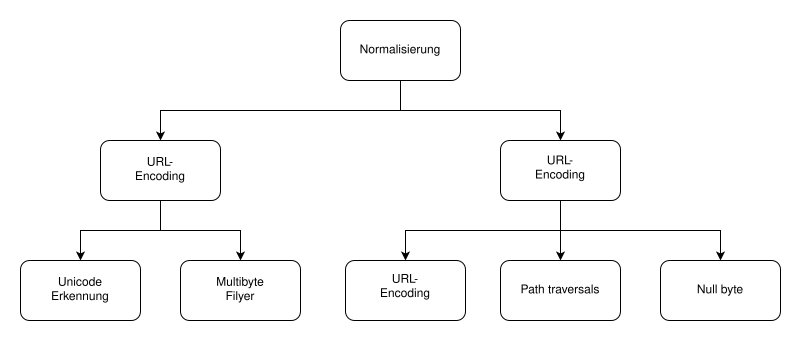
\includegraphics[width=0.9\textwidth]{./images/Normalisierung.png}
    \caption{Normalisierungsoperationen}
    \label{fig:norming}
\end{figure}

Normalisiert werden muss zum Einen die Zeichendarstellung.
Die Nachricht muss in ein einheilichs Encoding überführt werden, außerdem müssen \textit{URL-Encodings} aufgelöst werden.
Hier werden Sonderzeichen mit drei bytes dargestellt:
Das erste Zeichen ist immer ein \verb|%| gefolgt von einer Zahl in hexadezimaler Darstellung der das Zeichen repräsentiert.
Das \verb|@|-Zeichen wird von \verb|%40| repräsentiert, soll das Zeichen \verb|%| selber dargestellt werden muss dies mit \verb|%25| codiert werden.
Weitere Normalisierungsoperationen sind das Entfernen von Null Bytes.
Ein Null Byte ist ein Zeichen das nicht dargestellt wird.
Alle oben genannten Techniken können genutzt werden um nicht von regulären Ausdrücken erkannt werden zu können.

Eine weitere Gruppe von Normalisierungsoperationen sind Pfad-Normalisierungen.
Sollen Pfade nicht Normalisiert werden kann ein Angreifer Zugriff auf Verzeichnisse erlangen, die nicht zugänglich sein sollten.

Ist der Request Parsing Schritt abgeschlossen, liegt einen Nachricht in einer Form vor, die eine Einheitliche Analyse ermöglicht.

\paragraph{Muster-Abgleich gegen Regeln}
% - Abgleichen gegen Feature Datenbank
% - Jeder Parameter gegen jede regex
%     - Rechenaufwand
%         - optimierte regex-Engines
%         - Tree pruning
%             - Gefahr durch ungewollte pass on Szenarien
% - Whitelisting
%     - Features deaktivieren die web app-Funktion einschränken
% - Blacklisting
%     - Default Regelwerk
% - Auch Signatur-basierte WAFs
%     - komplexere Erkennung

Die normalisierte Nachricht kann von der \ac{waf} nun auf schädliche Inhalte untersucht werden.
In der Regel erfolgt das durch den Abgleich gegen eine Regel.
Eine Regel besteht aus einem regulären Ausdruck und einem Set an Instruktionen wie mit der Nachricht, im Fall das eine Übereinstimmung besteht, verfahren werden soll. 



\paragraph{Logging}
% - Jeder Schritt wird protokolliert
%     - Compliance
%         - Erfiltrierte Daten
%         - betroffene Nutzer
%     - Nachvollziehbarkeit von Fehlern
% - Log analyse
%     - Hauptarbeit eines WAF-Consultants

\paragraph{Weiteres Vorgehen}
% - Request Ablehnen
%     - Werden schädliche Daten erkannt
% - Request modifizieren
%     - Ablehnen bei schädlichen Inhalten nicht notwendig
%     - request kann umgeschrieben werden
%         - Abschnitte entfernen
%         - Abschnitte Escapeen
% - unmodofiziertes weiterleiten
% 
% - aus normalisierter form HTTP-Request erstellen
% - an server übergeben

\subsubsection{Erweiterte Funktionen}
\paragraph{Lernen von Regeln aus vorhergegangenem Datenverkehr}
\paragraph{KI-Features}
\subsubsection{Deployment einer WAF}
\paragraph{Postitionierung einer WAF}
\paragraph{Betrieb einer WAF}
\subsubsection{Schwächen und Nachteile einer WAF}
